\subsection[Komponenty systemu(Jakub Wyka)]{Komponenty sprzetowe}

\begin{tabular}{|p{2cm}|p{12cm}|}
    \hline
    \textbf{} & \textbf{Serwer} \\
    \hline
    Opis: & Serwer hostuje aplikację do zarządzania testami. \\
    \hline
    Powiązania: & Podsystem zarządzania \\
    \hline
    Priorytet: & wysoki \\ 
    \hline
\end{tabular}  
\label{tab:koms1}

\vskip 0.3cm

\begin{tabular}{|p{2cm}|p{12cm}|}
    \hline
    \textbf{} & \textbf{Platforma wykonująca} \\
    \hline
    Opis: & Mała platforma podłączana bezpośrednio do testowanego komputera i komunikująca się z serwerem. \\
    \hline
    Powiązania: & Podsystem wykonywania \\
    \hline
    Priorytet: & krytyczny \\ 
    \hline
\end{tabular}  
\label{tab:koms2}

\vskip 0.3cm

\begin{tabular}{|p{2cm}|p{12cm}|}
    \hline
    \textbf{} & \textbf{Platforma pentestera} \\
    \hline
    Opis: & Dowolna platforma mająca dostęp do internetu oraz przeglądarkę internetową. \\
    \hline
    Powiązania: & Podsystem prezentacji \\
    \hline
    Priorytet: & średni \\ 
    \hline
\end{tabular}  
\label{tab:kom3}

\begin{figure}[H]
    \centering
    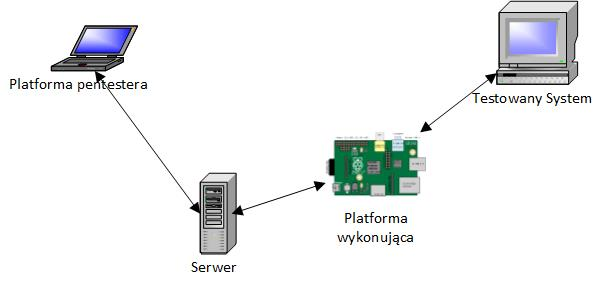
\includegraphics[width=\textwidth]{sprzet}
    \caption{Diagram komponentów sprzętowych}
    \label{fig:sprzet}
\end{figure}
